%=================================================================
\subsection{Example 2: W-N}
%=================================================================
\begin{frame}
  \frametitle{Example 2: W-N}

\begin{footnotesize}
\begin{block}{Data I}
1.208339 1.748644 2.080409 2.335513 2.548681 2.734928 2.902281
3.055600 3.198078 3.331945 3.458826 3.579955 3.696291 3.808603
3.917520 4.023568 4.127191 4.228776 4.328661 4.427151 4.524519
4.621021 4.716894 4.812366 4.907658 5.002987 5.098571 5.194633
5.291403 5.389125 5.488057 5.588484 5.690718 5.795109 5.902057
6.012024 6.125552 6.243292 6.366035 6.494765 6.630734 6.775576
6.931493 7.101568 7.290332 7.504885 7.757387 8.071660 8.506590
9.315591
\end{block}

\begin{block}{Data II}
\begin{color}{red}
0.923350 1.642687 2.049681 2.346765 2.586173 2.789748 2.968822
3.130079 3.277814 3.414961 3.543624 3.665370 3.781399 3.892659
3.999913 4.103790 4.204817 4.303443 4.400057 4.495004 4.588591
4.681098 4.772786 4.863899 4.954671 5.045329 5.136101 5.227214
5.318902 5.411409 5.504996 5.599943 5.696557 5.795183 5.896210
6.000087 6.107341 6.218601 6.334630 6.456376 6.585039 6.722186
6.869921 7.031178 7.210252 7.413827 7.653235 7.950319 8.357313
9.076650
\end{color}
\end{block}
\end{footnotesize}
%----------
\end{frame}


%% %%--------------------------------
\begin{frame}   %%[allowframebreaks]
\begin{figure}[h]
   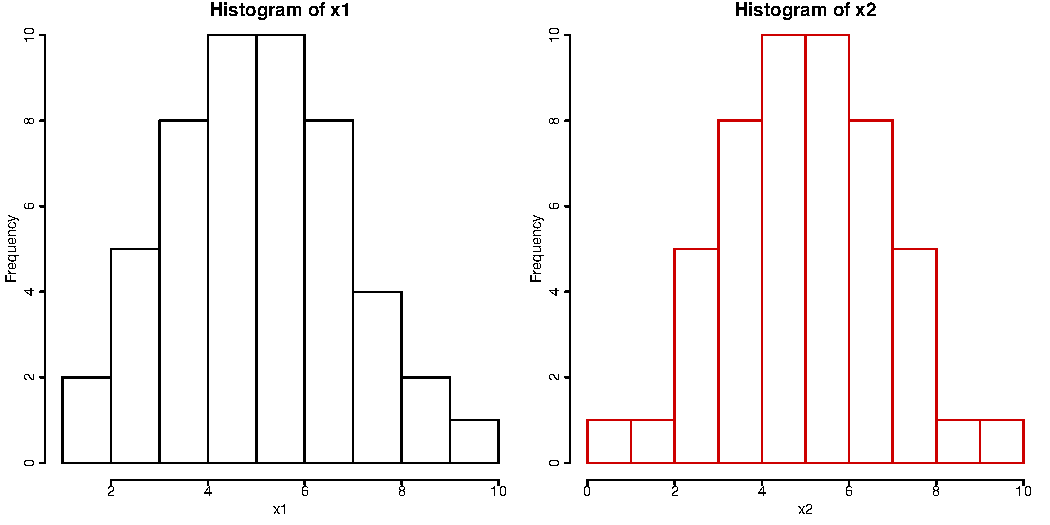
\includegraphics[width=4.5in]{hist2.pdf} %%-Figure (pdf file)
   \vspace{-3ex}
\end{figure}
\end{frame}
%% %%--------------------------------
% \begin{frame}   %%[allowframebreaks]
% \begin{figure}[h]
% %%  %% \centering\includegraphics{BPweibullplot.ps} %%-Figure (ps file)
%    \includegraphics[height=4.5in,angle=90]{CDF2a.pdf} %%-Figure (pdf file)
%    \vspace{-3ex}
% \end{figure}
% \end{frame}
% %% %%--------------------------------
% \begin{frame}   %%[allowframebreaks]
% \begin{figure}[h]
% %%  %% \centering\includegraphics{BPweibullplot.ps} %%-Figure (ps file)
%    \includegraphics[height=3.0in,angle=90]{CDF2b.pdf} %%-Figure (pdf file)
%    \vspace{-3ex}
% \end{figure}
% \end{frame}
%% %%---------------------------------------------------
\begin{frame}   %%[allowframebreaks]
\begin{figure}[h]
%%  %% \centering\includegraphics{BPweibullplot.ps} %%-Figure (ps file)
   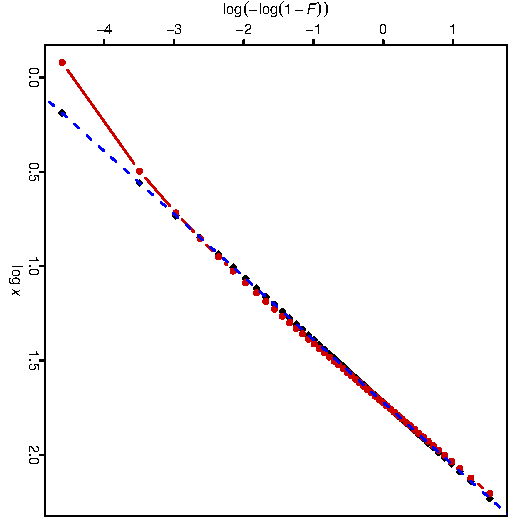
\includegraphics[width=3.0in,angle=90]{Weibull2.pdf} %%-Figure (pdf file)
   \vspace{-3ex}
\end{figure}
\end{frame}
%% %%---------------------------------------------------

